\documentclass{beamer}
%
% Choose how your presentation looks.
%
% For more themes, color themes and font themes, see:
% http://deic.uab.es/~iblanes/beamer_gallery/index_by_theme.html
%
\mode<presentation>
{
	\usetheme{Luebeck}      % or try Darmstadt, Madrid, Warsaw, ...
	\usecolortheme{dolphin} % or try albatross, beaver, crane, ...
	\usefonttheme{structuresmallcapsserif}  % or try serif, structurebold, ...
	\setbeamertemplate{navigation symbols}{}
	\setbeamertemplate{caption}[numbered]
} 

\usepackage[english]{babel}
\usepackage[utf8x]{inputenc}

\title[ESPN's Total QBR]{Investigation of ESPN's Total Quarterback Rating}
\author{Justin Gomez}
\institute{Montana State University}
\date{April 17, 2017}

\begin{document}
	
	\begin{frame}
		\titlepage
	\end{frame}
	
	% Uncomment these lines for an automatically generated outline.
	%\begin{frame}{Outline}
	%  \tableofcontents
	%\end{frame}
	
	\section{Introduction}
	
	\begin{frame}{Outline}
		\begin{columns}
			\column{0.5\textwidth}
			\begin{itemize}
				\item ESPN's Total QBR
				\item Variables and Models
				\item Methods
				\item Regression Trees
				\item Bagging
				\item Boosting
			\end{itemize}
			\column{0.5\textwidth}
			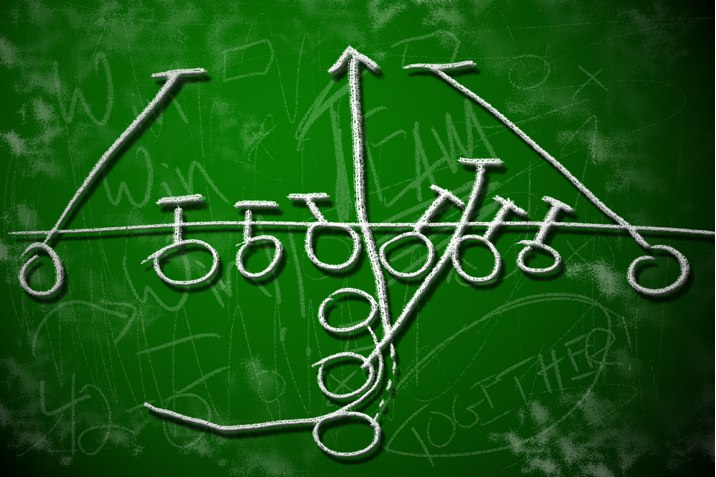
\includegraphics[scale=.2]{football-strategy.jpg}
		\end{columns}
	\end{frame}
	
	\begin{frame}{ESPN's Total QBR}
		\begin{columns}
			\begin{column}[t]{0.5\textwidth}
				Pros
				\begin{itemize}
					\item Intuitive scale (0-100)
					\item Utilizes a great deal of information
					\begin{itemize}
						\item Win Probability
						\item Expected Points
						\item Division of Credit
						\item Clutch Index
					\end{itemize}
				\end{itemize}
			\end{column}
			
			\begin{column}[t]{0.5\textwidth}
				Cons
				\begin{itemize}
					\item Complicated
					\item Vaguely explained
					\item Subjective
					\item Proprietary
				\end{itemize}
			\end{column}
		\end{columns}
	\end{frame}

	\begin{frame}{Variables}
	Seven Predictors:
	\begin{itemize}
		\item Completion Percentage (compp)
		\item Number of interceptions (int)
		\item Number of fumbles (fum)
		\item Total yards (yds)
		\item Game result (result)
		\item Number of sacks (sack)
		\item Total touchdowns (td)
		\end{itemize}
	\end{frame}

	%\begin{frame}{Variables and Models}
		%\vspace{-4pt}
		%\begin{columns}
			%\column{\dimexpr\paperwidth-20pt}
			%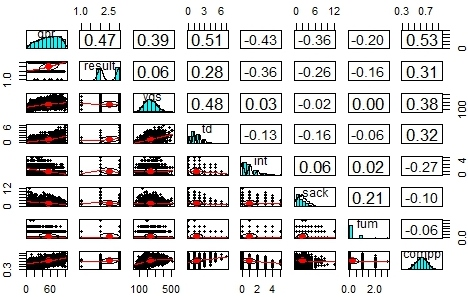
\includegraphics[scale=.95]{variablespanels.jpeg}
		%\end{columns}
	%\end{frame}
	
	\section{Methods}
	
	\begin{frame}{Methods Overview}
		Four modeling techniques:
		\begin{itemize}
			\item Linear models
			\item Generalized additive models
			\item Regression trees
			\item Random forests
		\end{itemize}
		Two improvement algorithms:
		\begin{itemize}
			\item Bootstrap Aggregating (bagging)
			\item Boosting
		\end{itemize}
	\end{frame}

	\begin{frame}{Regression Trees}
		Primary goal: partitioning the predictor space
		\vspace{20pt}
		\begin{columns}
			\begin{column}[t]{0.5\textwidth}
				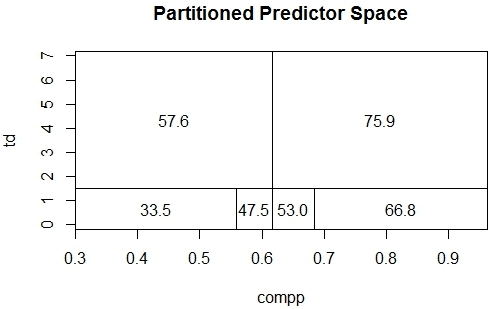
\includegraphics[scale=.45]{expartspace.jpeg}
			\end{column}
			\begin{column}{0.08\textwidth}
			\end{column}
			\begin{column}[t]{\dimexpr\paperwidth-20pt}
				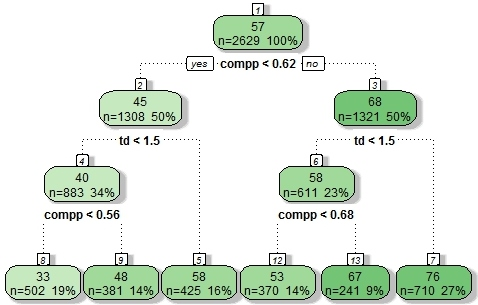
\includegraphics[scale=.5]{extree.jpeg}
			\end{column}
		\end{columns}
	\end{frame}

	\begin{frame}{Bootstrap Aggregation}
		\begin{columns}
			\begin{column}{0.5\textwidth}
				\begin{itemize}
					\item High level algorithm:
					\begin{itemize}
						\item Obtain bootstrap sample
						\item Grow regression tree
						\item Use tree to predict values\\
						for new observations
						\item Repeat n times
						\item Aggregate predictions 
					\end{itemize}
					\item Benefits:
					\begin{itemize}
						\item Prediction variance reduced
						\item More accurate
						\item Helps avoid overfitting
					\end{itemize}
				\end{itemize}
			\end{column}
			\begin{column}{0.5\textwidth}
				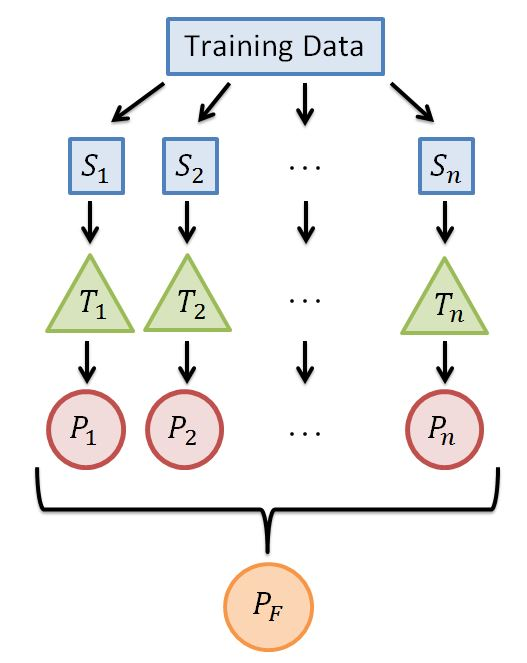
\includegraphics[scale=.4]{baggingalg.jpg}
			\end{column}
		\end{columns}
	\end{frame}

	\begin{frame}{Boosting}
		\begin{itemize}
			\item Performed on full training set
			\item Slow learning algorithm
			\item Typically performs better than a random forest
			\item High level algorithm:
			\begin{itemize}
				\item Grow tree with training set
				\item Predict values for new observations
				\item Find residuals for predictions
				\item Grow tree with residuals
				\item Repeat n times
			\end{itemize}
		\end{itemize}
		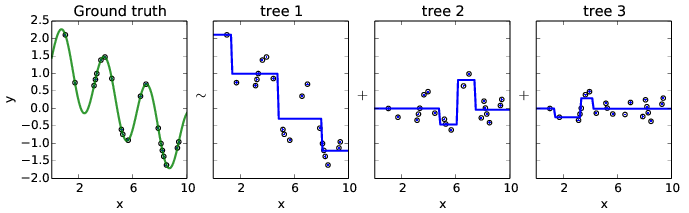
\includegraphics[scale=.4]{boostingex.png}
	\end{frame}
	
	\section{Results}
	
	\begin{frame}{Choosing the Best Performer}
		\begin{itemize}
			\item Models judged and compared according to RMSE
		\end{itemize}
		%\begin{equation}
			%RMSE=\sqrt{\frac{\sum_{i=1}^{n}(\hat{y_{i}}-y_{i})^{2}}{n}
		%\end{equation}		
	\end{frame}
	
\end{document}
